\section{Implementation Details}
As mentioned earlier, DeputyDev can integrate with popular version control systems like Github, Gitlab and Bitbucket. When a pull request is raised, DeputyDev receives an event through webhook. Automated review then starts in the background without interfering with the developer's usual workflow.

Upon receiving this pull request event, DeputyDev starts to create optimized context as mentioned above by leveraging its integration with version control systems and Atlassian suite

\subsection{Retrieving contextually relevant code chunks}
Everytime a pull request event is received by DeputyDev, It clones the repository ephemerally, create Abstract Syntax Trees(AST) out of it and semantically chunk the ASTs. This process of breaking down the code into meaningful, logical segments based on their functionality, purpose, or conceptual relationships, rather than just arbitrary divisions. Each chunk is provided with a unique ID and is stored in the redis cache with a specified TTL.

After performing chunking of the codebase several types of searches including lexical and semantic search is performed on the set of chunks. These searches is performed by using PR diff as a search query. Search results then received are merged together to obtain contextually relevant code chunks.

Example - If $R_{LS}$ is set of code chunks retrieved by lexical search and $R_{SS}$ is set of code chunks retrieved by semantic search then -

$R_f = (R_{LS} \cup R_{SS})$

Where, $R_f$ is final set of contextually relevant code chunks\ref{fig:DeputyDev-search}

Now that we have all the pieces of information we need to create optimized context, the next step would be to call LLMs with this context to get a response.

\subsection{Agentic workflow}
DeputyDev uses agentic workflow to further optimize the quality and better segregate responsibilities of different aspects of the code review process. Inspired by Andrew Ng's letters \cite{deeplearningFourAgent}, DeputyDev's agentic workflow is an amalgamation of 2 agentic design patterns i.e. Multi-agent and Reflection.

An agentic workflow is different from a comprehensive workflow where optimized context is passed on to LLM to obtain review on all aspects of code in a single pass. In an agentic workflow, we define agents to cater to each specific aspect. There are pros and cons to agentic design which are as follows-

\subsubsection{Benefits of Agentic Workflow}
\begin{enumerate}
    \item \textbf{Attention and Working Memory}: AI models, like humans, have limitations in their "working memory" (in this case, the context window). By focusing on one aspect at a time, the model can dedicate more of its processing capacity to that specific task, potentially leading to more thorough and nuanced analysis.
    \item \textbf{Task Complexity}: Code review involves multiple complex subtasks. Breaking these down into separate focused reviews aligns with the principle of divide-and-conquer in problem-solving, which often leads to better results in complex tasks.
    \item \textbf{Prompt Engineering}: This method allows for more specific and detailed prompts for each aspect, which can guide the model's attention more effectively. This is similar to how specific questions often elicit more precise and useful responses in human communication.
    \item \textbf{Iterative Improvement}: This method allows for iterative refinement of prompts based on the results of each focused review, potentially leading to better overall outcomes.
    \item \textbf{Parallel Processing}: Agents can work simultaneously on different aspects of the code, potentially reducing overall review time.
    \item \textbf{Customizable Reviews}: Users can choose which agents to activate based on their specific needs or project requirements.
    \item \textbf{Clearer Reporting}: Issues can be categorized more effectively, making it easier for developers to understand and address feedback.
    \item \textbf{Continuous Improvement}: Individual agents can be updated or fine-tuned without affecting the entire system.
\end{enumerate}

\subsubsection{Drawbacks of Agentic Workflow}
\begin{enumerate}
    \item \textbf{Increased Complexity}: Managing multiple agents adds complexity to the system architecture and maintenance.
    \item \textbf{Increased Inference cost}: Multiple agents means all of them will have their own optimized context. This will surely increase the number of input tokens and may increase the number of output tokens.
    \item \textbf{Potential Redundancy}: Agents might overlap in their analyses, leading to duplicate findings or conflicting advice.
    \item \textbf{Integration Challenges}: Ensuring smooth communication and coordination between agents may be challenging.
    \item \textbf{Higher Resource Usage}: Running multiple agents may require more computational resources compared to a single, comprehensive review.
\end{enumerate}

After carefully considering the advantages and disadvantages of an agentic workflow, we decided to upgrade to a generic design approach from a comprehensive approach as it is superior for achieving optimal quality. Consequently, we decided to implement an agentic workflow strategy.

Let's discuss agentic design patterns we used-

\begin{figure*}[htbp]
    \centering
    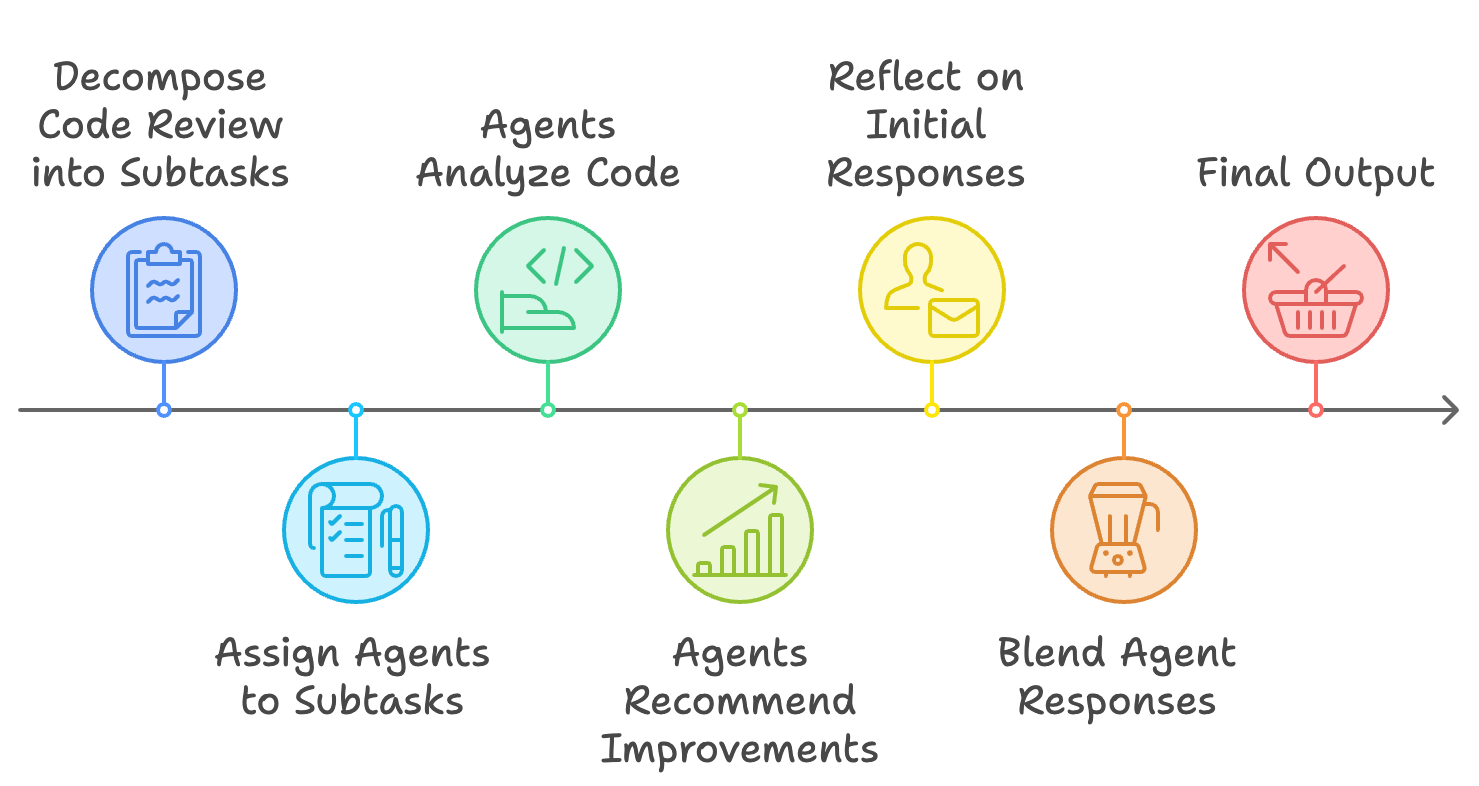
\includegraphics[width=0.8\textwidth]
    {Figures/workflow.png}
    \caption{DeputyDev workflow using multi-agent and reflection design patterns before blending the results together.}
    \label{fig:DeputyDev-workflow}
\end{figure*}


\subsubsection{Multi-Agent design pattern}
\textit{"Even though some LLMs today can accept very long input contexts (for instance, Gemini 1.5 Pro accepts 1 million tokens), their ability to truly understand long, complex inputs is mixed. A multi-agentic workflow in which the LLM is prompted to focus on one thing at a time can give better performance. By telling it when it should play software engineer, we can also specify what is important in that role's subtask. For example, the prompt above emphasized clear, efficient code as opposed to, say, scalable and highly secure code. By decomposing the overall task into subtasks, we can optimize the subtasks better."} - Andrew Ng \cite{deeplearningAgenticDesign}

We decompose our task of reviewing code into smaller subtasks. Each subtask being handled by an agent of its own. \cite{qian2024chatdevcommunicativeagentssoftware} Following are the agents we defined-

\begin{enumerate}
    \item \textbf{Security}: This agent is responsible to identify and recommend corrective code for any security issues it observes in the code. This could be issues like Injection attacks, Improper input validation, Using components with known vulnerabilities, Hardcoded credentials etc.
    \item \textbf{Code communication}: This agent is responsible to identify issues with aspects like documentation, docstring and logging. This could be issues like missing/incomplete docstrings, Improper documentation for a snippet. Incorrect or inconsistent logging usage etc.
    \item \textbf{Performance optimizations}: This agent is responsible to identify issues specifically related to performance issues and suggest optimisations on them. This will include algorithmic optimisations to reduce space \& time complexity, database query optimizations and other forms of code optimisation best practices.
    \item \textbf{Code maintainability}: This agent is responsible to identify issues pertaining to code maintainability, readability, reusability and quality.
    \item \textbf{Errors}: This agent is responsible to identify any logical, syntactical or runtime error that the change may induce.
    \item \textbf{Business validation}: This agent is responsible for correlating changes being done in PR to actual business requirements. It checks if changes adhere to stated requirements or not.
\end{enumerate}

\begin{table*}[ht]
\centering
\caption{List of agents along with which piece of information constitutes to make optimized context.}
\label{tab:agent-prompt-matrix}
\small
\begin{tabularx}{\textwidth}{@{}l*{7}{>{\centering\arraybackslash}X}@{}}
\toprule
Agent & PR Diff & PR Title & PR Description & Context Code & User Story & Confluence Pages & Initial LLM Review \\
\hline
Security & $\checkmark$ & $\checkmark$ & $\checkmark$ & & & & $\checkmark$ (Refl.) \\
Code Communication & $\checkmark$ & $\checkmark$ & $\checkmark$ & & & & $\checkmark$ (Refl.) \\
Performance Optimization & $\checkmark$ & $\checkmark$ & $\checkmark$ & $\checkmark$ & & & $\checkmark$ (Refl.) \\
Code Maintainability & $\checkmark$ & $\checkmark$ & $\checkmark$ & $\checkmark$ & & & $\checkmark$ (Refl.) \\
Error & $\checkmark$ & $\checkmark$ & $\checkmark$ & $\checkmark$ & & & $\checkmark$ (Refl.) \\
Business Logic Validation & $\checkmark$ & $\checkmark$ & $\checkmark$ & $\checkmark$ & $\checkmark$ & $\checkmark$ & $\checkmark$ (Refl.) \\
\bottomrule
\end{tabularx}
\end{table*}

\subsubsection{Reflection design pattern}
\textit{"Today, we mostly use LLMs in zero-shot mode, prompting a model to generate final output token by token without revising its work. This is akin to asking someone to compose an essay from start to finish, typing straight through with no backspacing allowed, and expecting a high-quality result. Despite the difficulty, LLMs do amazingly well at this task!"} - Andrew Ng \cite{deeplearningFourAgent}

Reflection in the context of large language models (LLMs) refers to the ability of an AI system to analyze and think about its own thought processes, outputs, and performance. This concept aims to make AI models more self-aware and capable of improving their own responses. \cite{shinn2023reflexionlanguageagentsverbal}  \cite{madaan2023selfrefineiterativerefinementselffeedback} Here are some key aspects of reflection in LLMs:

\begin{enumerate}
    \item \textbf{Self-evaluation}: The model assesses the quality, accuracy, and appropriateness of its own outputs.
    \item \textbf{Iterative improvement}: Based on self-evaluation, the model can refine and improve its responses.
    \item \textbf{Metacognition}: The ability to think about its own thinking process, including recognizing limitations or potential biases.
    \item \textbf{Error detection}: Identifying mistakes or inconsistencies in its own reasoning or outputs.
    \item \textbf{Confidence assessment}: Evaluating how certain the model is about different parts of its response.
\end{enumerate}

Upon receiving the initial response from LLMs, we send it back to LLM with its initial response and ask it to reflect on it. LLM then responds back with a higher quality response. This is done for each agent in order to achieve higher quality output.

GPT-3.5 (zero shot) was 48.1\% correct. GPT-4 (zero shot) does better at 67.0\%. However, the improvement from GPT-3.5 to GPT-4 is dwarfed by incorporating an iterative agent workflow. Indeed, wrapped in an agent loop, GPT-3.5 achieves up to 95.1\% \cite{deeplearningFourAgent}

% Insert Figure-6 here to show which pieces of context are passed to which agent


\subsection{Structured/Unstructured output}
LLMs output are string or stream of strings. To use LLM responses for anything meaningful in industrial grade applications, a structured (JSON/XML) output is required for it to be successfully parsed by code. Developers have long been working around the limitations of LLMs in this area via open source tooling, prompting, and retrying requests repeatedly to ensure that model outputs match the formats needed to interoperate with their systems.

OpenAI and Anthropic models already have a JSON mode hyperparameter which can be turned on to expect a JSON response. While JSON mode improves model reliability for generating valid JSON outputs, it does not guarantee that the model's response will conform to a particular schema. OpenAI recently introduced structured output in its API \cite{Introduc39:online}

It is however noticed that enforcing schema restriction on LLM's response results in significant drop in LLM's reasoning capabilities. \cite{tam2024letspeakfreelystudy} Thus, it is required to request LLMs without any schema restrictions and separate out the process of enforcing schema from the reasoning step.

Refer to Appendix \ref{app:agent_output_schema} for a LLM agent's response when schema restriction is enforced

\subsection{Blending engine}
Blending engine ($\Sigma$) is an integral part of DeputyDev's agentic workflow. It acts as a consolidator of final comments to be made on the pull request. Moreover, It provides us ways and measures by which we can filter in/out and fine tune the final comments.

Upon receiving responses from all the agents, all responses are unionized and passed on to the blending engines. Blending engine has the capability to house dimensions in it. These dimensions are basically a set of rules that each agentic response should follow. As a result of running each dimension, comments can be filtered in/out or modified. This is done to achieve higher quality response and reduce noise in most cases.

Following are some dimensions of blending engine-

\begin{enumerate}
    \item \textbf{Confidence score}: With the help of prompt engineering we are able to instruct LLMs to respond back with a confidence score with each comment. This is basically LLMs self confidence in the comment it is returning. This is a relatively simple dimension where we filter out all comments having a confidence score below some value X. This value X varies between agents depending on its weightage.
    \item \textbf{Comment overlap summarisation}: There can be a case where multiple agents provide their respective comments on the same line of a file. This can add noise for the reviewers and authors of the PR. This dimension summarizes all overlapping comments into one.
\end{enumerate}

\subsection{Mathematical modeling of agentic design}
To structure our agents, we refer communicative agents \cite{qian2024chatdevcommunicativeagentssoftware}

\begin{enumerate}
    \item $R_f$ is the final output (a list of comments that DeputyDev will make on the PR)
    
    $R_f = \Sigma\langle A_1, A_2, ..., A_n\rangle$
    
    \begin{itemize}
        \item Where $A_i$ is an agent responsible for performing review on PR from a specific perspective like security, code quality etc. Agents are mutually exclusive and can be executed in parallel.
        \item $\Sigma$ refers to a blending engine which acts as a post-processing module and consolidates (filter in/out) comments basis some predefined dimensions/factors like confidence score etc.
    \end{itemize}
    
    \item $A_i = C\langle R_{sp}, R_r\rangle$
    \begin{itemize}
        \item Where C is a consensus reached between $R_{sp}$ (Single pass response from LLM) and $R_r$ (Reflection response from LLM)
    \end{itemize}
    
    \item $C\langle R_{sp}, R_r\rangle = \langle DD \rightarrow LLM, LLM ; DD\rangle_{sp} | \langle DD \rightarrow LLM, LLM ; DD\rangle_r$
    \begin{itemize}
        \item Where DD is DeputyDev and LLM can be any large language model. Claude 3.5 Sonnet in our case.
        \item This means DD submits a prompt to LLM $\langle DD \rightarrow LLM\rangle$ and LLM responds back to DD $\langle LLM ; DD\rangle$
        \item Subscripted sp and r means Single pass (1st request to LLM) and reflection response respectively. Pipe $ \pipe $ represents reflection. It means Single pass response is fed back to LLM as context to attain structured and higher quality response.
        \item Reflection in this case serves 2 objectives-
        \begin{itemize}
            \item Self reflect on LLM's response and correct the response against any anomalies. It increases the quality of response.
            \item Converting unstructured response to structured response for DD to consume.
        \end{itemize}
    \end{itemize}
\end{enumerate}